%=======================================================

%<*typedgraphtext>

We will start by introducing the notion of typed graph. A typed graph is the essential object we will use throughout our mathematical development. Typed graphs will be used to formalise all the important graph-like structures we will present in this paper. A typed graph is a directed multigraph (a graph allowing multiple edges between two vertices) where vertices and edges are typed.

%</typedgraphtext>

%<*typedgraph>

A typed graph is a 6-tuple $\langle V,E,(s,t),\tau, VT, ET\rangle$ where: $V$ is a finite set of vertices; $E$ is a finite set of directed edges connecting the vertices $V$; $(s,t)$ is a pair of functions $s: E\rightarrow V$ and $t: E\rightarrow V$ that respectively provide the source and target vertices for each edge in the graph; function $\tau:V\cup E\rightarrow VT \cup ET$ is a typing function for the elements of $V$ and $E$, where $VT$ and $ET$ are disjoint finite sets of vertex and edge type identifiers and $\tau(v)\in VT$ if $v\in V$ and $\tau(e)\in ET$ if $e\in E$. Edges $e\in E$ are noted $v\xrightarrow{e} v'$ if $s(e)=v$ and $t(e)=v'$, or simply \emph{e} if the context is unambiguous. The set of all typed graphs is called $\textsc{Tg}$. 

%</typedgraph>

%=======================================================

%<*typedgraphuniontext>

We now define how two typed graphs are united. A union of two typed graphs is trivially the set union of all the components of those two typed graphs. Note that we do not require the components of the two graphs to be disjoint, as in the following joint unions will be used to merge typed graphs.

%</typedgraphuniontext>

%<*typedgraphunion>
Let $\langle V,E,(s,t),\tau,VT,ET\rangle,\langle V',E',(s',t'),\tau',VT',ET'\rangle\in \textsc{Tg}$ be typed graphs, where $VT$ and $ET'$ are disjoint sets, as well as $VT'$ and $ET$. The typed graph union is the function $\sqcup :\textsc{Tg}\times \textsc{Tg}\rightarrow \textsc{Tg}$ defined as:
\begin{multline*}
\big\langle V,E,(s,t),\tau,VT,ET\big\rangle\;\sqcup\;\big\langle V',E',(s',t'),\tau',VT',ET'\big\rangle=\\\big\langle V\cup V', E\cup
E',(s\cup s', t\cup t'), \tau\cup \tau', VT\cup VT', ET\cup ET'\big\rangle
\end{multline*}
%</typedgraphunion>

%=======================================================

%<*typedgraphhomomorphismtext>

For the formal development of our technique, we are interested in relations between typed graphs that are structure-preserving, i.e. homomorphisms. Homomorphisms between typed graphs preserve not only structure, but also the types of vertices and edges that are mapped.

%</typedgraphhomomorphismtext>

%<*typedgraphhomomorphism>
Let $\langle V,E,st,\tau,VT,ET\rangle=g$ and $\langle V',E',st',\tau',VT',ET'\rangle=g'\in \textsc{Tg}$ be typed graphs. A typed graph homomorphism between $g$ and $g'$ is a function $f:V\rightarrow V'$ such that for all $v_1 \xrightarrow{e} v_2\in E$ we have that $f(v_1) \xrightarrow{e'} f(v_2)\in E'$, where $\tau(v_1)=\tau'(f(v_1))$, $\tau(v_2)=\tau'(f(v_2))$ and also $\tau(e)=\tau(e')$. The domain of $f$ is noted $Dom(f)$ and the co-domain of $f$ is noted $CoDom(f)$. When an \emph{injective} typed graph homomorphism $f$ exists between $g$ and $g'$ we write $g \stackrel{f}{\vartriangleleft} g'$, or simply $g \vartriangleleft g'$ when the context is unambiguous. When a \emph{surjective} typed graph homomorphism $f$ exists between typed graphs $g$ and $g'$ we write $g \stackrel{f}{\blacktriangleleft} g'$, or also simply $g \blacktriangleleft g'$ in an unambiguous context. 
%</typedgraphhomomorphism>

%=======================================================


%<*typedsubgraphtext>

We now define the useful notion of typed subgraph. As expected, a typed subgraph is simply a restriction of a typed graph to some of its vertices and edges.  

%</typedsubgraphtext>

%<*typedsubgraph>
Let $\langle V,E,st,\tau,VT,ET\rangle=g,\langle V',E',st,\tau',VT',ET'\rangle=g'\in \textsc{Tg}$ be typed graphs. $g'$ is a typed subgraph of $g$, written $g'\sqsubseteq g$, iff $V'\subseteq V$, $E'\subseteq E$ and $\tau'=\tau |_{V'\cup E'}$.
%</typedsubgraph>

%=======================================================

%<*typedgraphisomorphismtext>

Two typed graphs are said to be isomorphic if they have exactly the same shape and related vertices and edges have the same type.

%</typedgraphisomorphismtext>

%<*typedgraphisomorphism>
Let $\langle V,E,st,\tau,VT,ET\rangle=g,\langle V',E',st',\tau',VT',ET'\rangle=g'\in \textsc{Tg}$ be typed graphs. We say that $g$ and $g'$ are isomorphic, written $g\cong g'$, if and only if there exists a bijective typed graph homomorphism $f:V\rightarrow V'$ such that $f^{-1}:V'\rightarrow V$ is a typed graph homomorphism.
%</typedgraphisomorphism>

%=======================================================

%<*notationformalbackground>
In order to simplify our notation, when the context is unambiguous we will abbreviate a typed graph $\langle V,E,st,\\\tau,VT, ET\rangle$ as as 4-tuple $\langle V,E,st,\tau\rangle$. Also, given a typed graph $g\in \textsc{Tg}$, will use the notation $Components(g)$ to describe the set of strongly connected typed graphs in $g$. Finally, we will use the notation $g|_{t}$ to refer to the restriction of graph $g$ to its subgraph containing only edges of type $t$.
%</notationformalbackground>

%=======================================================

%<*metamodel>

A metamodel is a 5-tuple $\langle V,E,st,\tau,\leq\rangle$ where $\langle V,E,st,\tau\rangle\in \textsc{Tg}$ is a typed graph, $(V,\leq)$ is a partial order and $\tau$ is a bijective typing function. Additionally we also have that: if $v\in V$ then $\tau(v)\in VT\times \{abstract,concrete\}$, where $VT$ is the set of vertex type names; if $e\in E$ then $\tau(e)\in ET\times \{containment,\\reference\}$, where $ET$ is a set of edge type names. The set of all metamodels is called $\textsc{Meta}$.

%</metamodel>

%<*metamodeltext>

A formal metamodel is a particular kind of typed graph where vertices represent classes and edges represent relations between those classes. A typed graph representing a metamodel has two special characteristics: on the one hand, the typing function for vertices and edges is bijective. This means that each type occurs only once in the metamodel, as is to be expected. On the other hand, a metamodel is equipped with a partial order between vertices. This partial order is used to model inheritance at the level of the metamodel's classes. Note that here we have overridden the co-domain of the typing function in the original typed graph presented in \cref{def:typed_graph} in order to allow distinguishing between \emph{abstract} and \emph{concrete} classes, as well as between \emph{containment} and \emph{reference} edges in our metamodels. For simplification purposes, we do not model association cardinalities in our formal notion of metamodel as cardinalities are not strictly necessary in our development.

%\levi{Cardinalities are not treated, meaning all relations can be n-to-m. It may be necessary to treat cardinalities.}

%</metamodeltext>

%<*metamodeltextappendix>

A formal metamodel is a particular kind of typed graph where vertices represent classes and edges represent relations between those classes. A typed graph representing a metamodel has two special characteristics: on the one hand, the typing function for vertices and edges is bijective. This means that each type occurs only once in the metamodel, as is to be expected. On the other hand, a metamodel is equipped with a partial order between vertices. This partial order is used to model specialization at the level of the metamodel's classes. Note that here we have overridden the co-domain of the typing function in the original typed graph presented in \cref{def:typed_graph_appendix} in order to allow distinguishing between \emph{abstract} and \emph{concrete} classes, as well as between \emph{containment} and \emph{reference} edges in our metamodels. For simplification purposes, we do not model association cardinalities in our formal notion of metamodel as cardinalities are not strictly necessary in our development. 

%\levi{Cardinalities are not treated, meaning all relations can be n-to-m. It may be necessary to treat cardinalities.}

%</metamodeltextappendix>

%=======================================================


%<*expandedmetamodel>


Let $mm = \langle V,E,st,\tau,\leq\rangle\in \textsc{Meta}$ be a metamodel. The expansion of $mm$, noted $mm^{\star}$, is a typed graph $\langle V',E',st',\tau'\rangle\in \textsc{Tg}$ built as follows:
\begin{itemize}
  \item $V' = V\setminus \{v\in V\,|\,\tau(v)=(\cdot\footnote{In our mathematical development we use a `dot' notation to represent that we do not care about the value of a particular variable in a given context.},abstract)\}$;
  \item $v_1\xrightarrow{e}v_2\in E'$ if $v_1\xrightarrow{e}v_2\in E$ and $\tau(v_1)=(\cdot,concrete)$ and $\tau(v_2)=(\cdot,concrete)$;
  \item if $v_1\xrightarrow{e}v_2\in E$ we have that $v'_1\xrightarrow{e'}v'_2\in E'$, where $v'_1\leq v_1$, $v'_2\leq v_2$ and $\tau'(e') = \tau(e)$;
  \item for all $v\in V'$ and $e\in E'$ we have that $\tau'(v)=\tau(v)$ and that $\tau'(e)=\tau(e)$.
%   \item $(v,(tv,concrete))\in \tau'$ if $(v,(tv,concrete))\in \tau$ (where $tv$ is a vertex type);
%   \item $(v_1\xrightarrow{e}v_2,(te,concrete))\in \tau'$ if $(v_1\xrightarrow{e}v_2,(te,concrete))\in \tau$ ($te$ ia an edge type).
\end{itemize}
%The set of all expanded metamodels in called $META^{\star}$.

%</expandedmetamodel>

%<*expandedmetamodeltext>


An expanded metamodel is an auxiliary construct where all the relations between types of a metamodel are made explicit, rather than remaining implicit in the specialization hierarchy. It is built by adding to the original metamodel typed graph a relation of type $t$ between two classes of the metamodel, whenever those classes specialize two classes that are also related by a relation of type $t$. Abstract classes and their relations do not carry over to the expanded metamodel. Expanded metamodels will be used in the subsequent text to facilitate formal the treatment of any structure involving polymorphism.

% Definition~\ref{def:metamodel} formally states that a metamodel corresponds to a graph of typed elements where only one element for each type is represented. This definition is then used to state definition~\ref{def:pattern}, where a typed graph is combined with its metamodel.

%</expandedmetamodeltext>

%=======================================================

%<*metamodelinstance>

An instance of a metamodel $mm = \langle V',E',st',\tau',\leq\rangle\in \textsc{Meta}$ is a typed graph $\langle V,E,st,\tau\rangle\in \textsc{Tg}$, where the co-domain of $\tau$ equals the co-domain of $\tau'$. Also, there is a typed graph homomorphism $f:V\rightarrow V'$ from $\langle V,E,st,\tau\rangle$ to the expanded metamodel $mm^{\star}$ and the graph $\big\langle V,\{e\in E\,|\,\tau(e)=(\cdot,containment)\}\big\rangle$ is acyclic. The set of all instances for a metamodel $mm$ is called $\textsc{Instance}^{mm}$.

%</metamodelinstance>

%<*metamodelinstancetext>


A metamodel instance is a useful intermediate formal notion that lies between metamodel and model. The injective typed graph homomorphism between a metamodel instance and metamodel models multiple ``instances'' of objects and relations being typed by one single class or relation of the metamodel. Metamodel instances do not allow cyclic containment relations, as enforced by EMF. 

% It requires the acyclicity constraints as that is required through models, transformation rules, path conditions and properties. It can be used to define transformation rules and can be further refined to define models.

%</metamodelinstancetext>

%=======================================================

%<*instanceclosure>

The containment transitive closure of a metamodel instance $\langle V',E',st',\tau'\rangle\in \textsc{Instance}^{mm}$ is a typed graph $\langle V,E,st,\tau\rangle$ where we have that $V=V'$, $\tau' \supseteq \tau$ and $\tau$'s co-domain is the union of the co-domain of $\tau'$ and the set $\{indirect\}$. We also have that $E' = E\cup E^*_c$ where $E^*_c$ is the transitive closure of the set $\big\{v\xrightarrow{e}v'\,|\,\tau(v\xrightarrow{e}v') = (\cdot,containment)\big\}$ and if $e\in E\setminus E'$ then $\tau(e) = indirect$.  We denote $mi^{*}$ the containment closure of a metamodel instance $mi\in \textsc{Instance}^{mm}$.

%</instanceclosure>

%<*instanceclosuretext>


Given a metamodel instance, its containment transitive closure includes, besides the original graph, all the edges belonging to the transitive closure of containment links in that metamodel instance. The transitive edges are typed as \emph{indirect}. In the definitions that follow we will use the $*$ notation, as in \cref{def:instance_closure}, to denote the containment transitive closure of structures that directly or indirectly include metamodel instances. For example, $tg^{*}$ would represent the containment transitive closure of typed graph $tg$ wherever containment edges are found in the graph. Note that the $*$ notation is different from the $\star$ notation, introduced in \cref{def:expanded_metamodel} for an expanded metamodel.

% It requires the acyclicity constraints as that is required through models, transformation rules, path conditions and properties. It can be used to define transformation rules and can be further refined to define models.

%</instanceclosuretext>

%<*instanceclosuretextappendix>


Given a metamodel instance, its containment transitive closure includes, besides the original graph, all the edges belonging to the transitive closure of containment links in that metamodel instance. The transitive edges are typed as \emph{indirect}. In the definitions that follow we will use the $*$ notation, as in \cref{def:instance_closure_appendix}, to denote the containment transitive closure of structures that directly or indirectly include metamodel instances. For example, $tg^{*}$ would represent the containment transitive closure of typed graph $tg$ wherever containment edges are found in the graph. Note that the $*$ notation is different from the $\star$ notation, introduced in \cref{def:expanded_metamodel_appendix} for an expanded metamodel.

% It requires the acyclicity constraints as that is required through models, transformation rules, path conditions and properties. It can be used to define transformation rules and can be further refined to define models.

%</instanceclosuretextappendix>


%=======================================================

%<*model>

A model of a  metamodel $mm = \langle V',E',st',\tau',\leq\rangle\in \textsc{Meta}$ is a metamodel instance $\langle V,E,st,\tau\rangle\in \textsc{Instance}^{mm}$, such that: there exists an injective typed graph homomorphism $f:V\rightarrow V'$ from $\langle V,E,st,\tau\rangle$ to metamodel $mm^{\star}$ where, if $b\in V$ and there exists an edge $a'\xrightarrow{e'} f(b)\in E'$ where $\tau(e') = (t,containment)$, then we also have that $a\xrightarrow{e} b\in E$, $f(a) = a'$ and $\tau(e)=t$. The set of all models for a metamodel $mm$ is called $\textsc{Model}^{mm}$.

%</model>

%<*modeltext>

A model, as per \cref{def:model}, is a metamodel instance where all the containment relations are respected. This means that if an object that is contained (as per the metamodel) exists in the model, then the model will also contain an instance of that containment relation together with an object that contains it. Two models can be observed in \cref{fig:transformationexample}, which are respectively instances of the \emph{Organization language} and \emph{Gender language} found in \cref{fig:squadmetamodel}.\\
Note that the containment constraint does not necessarily lead to infinite models in the case of containment relations with the same source and target classes. In fact, if the cardinality of the target class is allowed to be zero, then it is not necessary that the containment relation is instantiated. For example, this is the case for the containment relation \emph{supervise} in the metamodel of~\cref{fig:OrganizationLanguage}.

%</modeltext>

%<*modeltextappendix>
A model, as per \cref{def:model_appendix}, is a metamodel instance where all the containment relations are respected. This means that if an object having a containment relation exists in the model, then the model will also contain an instance of that containment relation together with a contained object. Note that this constraint does not necessarily lead to infinite models in the case of containment relations with the same source and target classes. In fact, if the cardinality of the target class is allowed to be zero, then it is not necessary that the containment relation is instantiated. This is for example the case of the containment relation \emph{supervise} in the metamodel of~\cref{fig:OrganizationLanguage}.

% \begin{figure}[h!] \centering \includegraphics[scale=.5]{./figures/model_instance_example.pdf}
% 	\caption{An Example of a Model, instance of a Metamodel}
% 	\label{fig:model_instance_example}
% \end{figure}


%</modeltextappendix>

%=======================================================

%<*inputoutputmodel>

An input-output model is a 6-tuple $\big\langle V,E,(s,t),\tau,Input,\\Output\big\rangle$, where: $Input=\langle V',E',st',\tau'\rangle\in \textsc{Instance}^{sr}$ is a model; $Output=\langle V'',E'',st'',\tau''\rangle\in \textsc{Instance}^{tg}$ is a metamodel instance; $Input$ and $Output$ are disjoint. Additionally we have that $V=V'\cup V''$, $E\subseteq E'\cup E''$ and $\tau\subseteq \tau'\cup \tau''$, where the co-domain of $\tau$ is the union of the co-domains of $\tau'$ and $\tau''$ and the set $\{trace\}$. An edge $e \in E\setminus E'\cup E''$ is called a \emph{traceability link} and is such that $s(e)\in V''$, $t(e)\in V'$ and $\tau(e)=trace$. The set of all match-apply patterns for a source metamodel $sr$ and a target metamodel $tg$ is called $\textsc{Iom}^{sr}_{tg}$.

%</inputoutputmodel>

%<*inputoutputmodeltext>


% \levi{A match-apply model is the union of an input and output models, plus potential traceability links between those models. Traceability links are now typed using the typing function $\tau$. A traceability link it typed with type ``trace''. This makes the definitions shorter and more compact, which was mentioned by one of the reviewers of the paper. However, the fact that a match-apply model is now made up of models makes it that the input and the output of the transformation are always well-formed, meaning that the containment relation is always respected. It may be that a transformation does not always produce a model respecting the containment relation, which is a problem. This can be solved however if we only consider that well-formed transformations actually have semantics.}

An input-output model is an object we will use when defining the semantics of a DSLTrans model transformation in \cref{sec:DSLTrans_formal}. It is composed of two metamodel instances, one called the \emph{input} and the other one the \emph{output}. An input-output model allows the representation of intermediate operational states during the execution of a model transformation. It may include a particular type of edges called \emph{traceability links}, for keeping a history of which elements in the output model originated from which elements in the input model.

%</inputoutputmodeltext>

%<*inputoutputmodeltextappendix>

An input-output model is an object we will use when defining the semantics of a DSLTrans model transformation in \cref{sec:DSLTrans_formal}. It is composed of two metamodel instances, one called the \emph{input} and the other one the \emph{output}. An input-output model allows the representation of intermediate operational states during the execution of a model transformation. It may include a particular type of edges called \emph{traceability links}, for keeping a history of which elements in the output model originated from which elements in the input model.

%</inputoutputmodeltextappendix>

%=======================================================

%<*metamodelpattern>

A pattern of a metamodel $mm\in \textsc{Meta}$ is an instance of $mm$. Given a metamodel pattern $\langle V',E',st',\tau'\rangle\in \textsc{Instance}^{mm}$ we have that $\langle V,E,st,\tau\rangle$ is an \emph{indirect} pattern if $V=V'$, $E'\supseteq E$ and the co-domain of $\tau$ is the union of the co-domains of $\tau'$ and the set $\{indirect\}$. Also, if $e\in E\setminus E'$, then we have that $\tau(e)=indirect$. Given a metamodel $mm$, the set of all metamodel patterns for $mm$ is called $\textsc{Pattern}^{mm}$. The set of all indirect metamodel patterns for $mm$ is called $\textsc{Ipattern}^{mm}$.

%</metamodelpattern>

%<*metamodelpatterntext>


Metamodel patterns are introduced in \cref{def:metamodel_pattern} as an intermediate notion, formally equal to metamodel instances. An \emph{indirect} metamodel pattern is a metamodel pattern that includes edges typed as \emph{indirect}. Both structures will be used as building blocks in the construction of transformation-related structures in the upcoming text.

%</metamodelpatterntext>

%<*metamodelpatterntextappendix>


Metamodel patterns are introduced in \cref{def:metamodel_pattern_appendix} as an intermediate notion, formally equal to metamodel instances. An \emph{indirect} metamodel pattern is a metamodel pattern that includes edges typed as \emph{indirect}. Both structures will be used as building blocks in the construction of transformation-related structures in the upcoming text.

%</metamodelpatterntextappendix>

%=======================================================

%<*transformationrule>

A transformation rule is a 6-tuple $\big\langle V,E,(s,t),\tau, Match,\\Apply\big\rangle$, where: $Match=\langle V',E',st',\tau'\rangle\in \textsc{Ipattern}^{sr}$ such that: $Match\neq \epsilon$\footnote{We use the simplified $\epsilon$ notation to denote empty n-tuples structures.} is an non-empty indirect metamodel pattern; $Apply=\langle V'',E'',st'',\tau''\rangle\in \textsc{Pattern}^{tg}$ such that $Apply\neq\epsilon$ is a metamodel pattern; $Match$ and $Apply$ are disjoint. We also have that $V=V'\cup V''$, $E\subseteq E'\cup E''$ and $\tau\subseteq \tau'\cup \tau''$, where the co-domain of $\tau$ is the union of the co-domains of $\tau'$ and $\tau''$ and the set $\{trace\}$. An edge $e \in E\setminus E'\cup E''$ is called a \emph{backward link} and is such that $s(e)\in V''$, $t(e)\in V'$ and $\tau(e)=trace$. We additionally impose that there always exists a $v_1\in V''$ in the Apply part of the rule such that $\nexists e\,.\, v_1\xrightarrow{e} v_2$ and $\tau(e)=trace$, or that $E''$ is not empty. The set of all transformation rules for a source metamodel $sr$ and a target metamodel $tg$ is called $\textsc{Rule}^{sr}_{tg}$.

%</transformationrule>

%<*transformationruletext>

A transformation rule is the elemental block of a model transformation. Several transformation rules can be observed in the Police Station transformation in \cref{fig:dsltransformation}. A formal transformation rule includes a non-empty match pattern and a non-empty apply pattern (also known in the model transformation literature as a rule's \emph{left hand side} and \emph{right hand side}). The apply pattern of a rule always contains at least one apply element that is not connected to a backward link or an edge, meaning in practice that a rule will always produce something and not only match. A match pattern can include indirect links that are used to transitively match containment relations in a model. An apply pattern does not include indirect links as it is used only for the construction of parts of instances of a metamodel. A transformation rule includes backward links, as informally introduced in \cref{subsec:DSLTrans_constructs}. Backward links are formally typed as \emph{trace}.%This eases modeling matching rules on models  by the use of typed graph homomorphisms.

%</transformationruletext>

%=======================================================

%<*backmatchtransformationrule>

Let $rl = \big\langle V,E,st,\tau, Match,Apply\big\rangle$ be a transformation rule where $Match =\langle V_m, E_m, st_m, \tau_m\rangle$. We define $rl$'s matcher, noted $\Vert rl\Vert$, as the transformation rule $\big\langle V',E',st',\tau',Match,\\Apply'\big\rangle\sqsubseteq rl$ where $v_1\xrightarrow{e} v_2\in E'$ if and only if $v_1,v_2\in Match$ or $\tau(e)=trace$ and $V'=V_m\cup \big\{v_1\,|\,v_1\xrightarrow{e} v_2\in E \land \tau(e)=trace\big\}$.

%</backmatchtransformationrule>

%<*backmatchtransformationruletext>

%'transformation rule cref in text
introduces the notion of matcher for a transformation rule which consists solely of the match pattern of a rule and its backward links, if any. The matcher of a rule constitutes the complete pattern that a DSLTrans rule attempts to match over a input-output model during rule execution. Traceability links between input and output model elements generated during transformation execution are matched by transformation rules' backward links, as informally explained in \cref{subsec:DSLTrans_constructs}.

%</backmatchtransformationruletext>

%=======================================================

%<*expandedtransformationrule>

Let $rl = \big\langle V,E,st,\tau,Match,Apply\rangle \in \textsc{Rule}^{sr}_{tg}$ be a transformation rule where $Match = \langle V',E',st',\tau'\rangle$ and also we have that $sr =\langle V'',E'',st'',\tau'',\leq \rangle$. The expansion of $rl$, noted $rl^{\star}$ is a set of transformation rules built as follows:
\begin{itemize}
  \item $rl\in rl^{\star}$;
  \item $\big\langle V,E,st,\tau',Match,Apply\rangle\in rl^{\star}$ iff for all $v\in V'$ we have that $\tau'(v)\leq \tau(v)$.
\end{itemize}

%</expandedtransformationrule>

%<*expandedtransformationruletext>

The expansion of a transformation rule is a set of transformation rules. Each rule in that set includes a possible replacement of each of the classes in the match part of the original rule by one of its subtypes. Expanded transformation rules will be important such that polymorphism is correctly handled in the developments that follow.  
 
%\levi{A transformation rule expansion simply takes a rule and builds all possible rules where a rule element is replaced by one of its subtypes.}

%</expandedtransformationruletext>

%=======================================================


%<*layertransformation>

A layer is a finite set of transformation rules $l\subseteq \textsc{Rule}^{sr}_{tg}$. The set of all layers for a source metamodel $sr$ and a target metamodel $tg$  is called $\textsc{Layer}^{sr}_{tg}$. A model transformation is a finite list of layers denoted $[l_{1}::l_{2}::\ldots::l_{n}]$ where $l_{k}\in \textsc{Layer}^{sr}_{tg}$ and $1\leq k \leq n$, $n\in \mathbb{N}$. We also impose that for any pair of rules $rl_1,rl_2\in \bigcup_{1\leq k\leq n}l_k$, if $\Vert rl_1\Vert \cong rl$ and $rl\sqsubseteq \Vert rl_2\Vert $ then $rl_2$ appears in a layer later than $rl_1$ and the apply parts of $rl_1$ and $rl_2$ are not isomorphic. The set of all transformations for a source metamodel $s$ and a target metamodel $t$ is called $\textsc{Transf}^{sr}_{tr}$. 

% The expansion of a layer $l\subseteq RULE^{sr}_{tg}$, noted $l^{\star}$, is such that that if
% $rl\in l$ then $rl'\in l$ if $rl'\in rl^{\star}$. This means that if a
% transformation rule is present is the layer, its expansion is also part of the
% layer.

%</layertransformation>

%<*layertransformationtext>

\cref{def:layer_transformation} formalises the abstract syntax of a model transformation, introduced in \cref{sec:dsltrans}. An example of a model transformation can be observed in \cref{fig:dsltransformation}, the Police Station transformation. As expected, a formal DSLTrans transformation is composed of a sequence of layers where each layer is composed of a set of rules. The last condition of \cref{def:layer_transformation} imposes that, for any two pair of rules in the transformation, the matcher of the second rule never partially or totally subsumes (or contains) the matcher of the first rule, unless the second rule is in a subsequent layer and produces something more than the first rule. This condition avoids situations where the execution of a rule in a DSLTrans model transformation necessarily implies the execution of another rule (except for when rules having backward links necessarily execute because all their dependencies were created during the execution of previous layers).

%\levi{At the syntactic level we have not included the expansion of a layer in the transformation. This is done at the semantic level.}

%</layertransformationtext>

%<*layertransformationtextappendix>

\cref{def:layer_transformation_appendix} formalises the abstract syntax of a model transformation, introduced at the beginning of this section. An example of a model transformation can be observed in \cref{fig:dsltransformation}, the Police Station transformation. As expected, a formal DSLTrans transformation is composed of a sequence of layers where each layer is composed of a set of rules. The last condition of \cref{def:layer_transformation_appendix} imposes that, for any two pair of rules in the transformation, the matcher of the second rule never partially or totally subsumes (or contains) the matcher of the first rule, unless the second rule is in a subsequent layer and produces something more than the first rule. This condition avoids situations where the execution of a rule in a DSLTrans model transformation necessarily implies the execution of another rule (except for when rules having backward links necessarily execute because all their dependencies were created during the execution of previous layers).

%\levi{At the syntactic level we have not included the expansion of a layer in the transformation. This is done at the semantic level.}

%</layertransformationtextappendix>

%=======================================================

%<*notationtext>

% In order to achieve a uniform notation throughout the text that follows, when the context is unambiguous we refer to transformation rules (\cref{def:transformation_rule}) as normal typed graphs. We also naturally extend to transformation rules the typed graph operations introduced in \cref{sec:formal_background}. Finally, given a structure such as transformation rule $rl = \langle V,E,st,\tau,Match,Apply\rangle$, we will refer to the structure's components by using the component's name followed by the variable that holds the structure in between parenthesis. For example, we will write $V(rl)$ to designate the $V$ component of $rl$ or $Apply(rl)$ to designate $rl$'s $Apply$ component.

We naturally extend to transformation rules (\cref{def:transformation_rule}) and transformation executions (\cref{def:modeltransformation}) the typed graph operations introduced in \cref{sec:formal_background}.  Also, given a structure such as transformation rule $rl = \langle V,E,st,\tau,Match,\\Apply\rangle$, we will refer to the structure's components by using the component's name followed by the variable that holds the structure in between parenthesis. For example, we will write $V(rl)$ to designate the $V$ component of $rl$ or $Apply(rl)$ to designate $rl$'s $Apply$ component.

% We will also use the natural extensions of the notions of typed graph union `$\sqcup$' (\cref{def:typed_graph_union}), typed graph homomorphism `$\vartriangleleft, \blacktriangleleft$' (\cref{def:typed_graph_homomorphism}), typed subgraph `$\sqsubseteq$' (\cref{def:typedsubgraph}) and typed graph isomorphism `$\cong$' (\cref{def:typed_graph_isomorphism}) to transformation rules.

%</notationtext>

%<*notationtextappendix>

We naturally extend to input-output models~(\cref{def:input_output_model_appendix}), transformation rules (\cref{def:transformation_rule_appendix}) and transformation executions (\cref{def:modeltransformation_appendix}) the typed graph operations introduced in \cref{sec:formal_background}. Also, given a structure such as transformation rule $rl = \langle V,E,st,\tau,Match,Apply\rangle$, we will refer to the structure's components by using the component's name followed by the variable that holds the structure in between parenthesis. For example, we will write $V(rl)$ to designate the $V$ component of $rl$ or $Apply(rl)$ to designate $rl$'s $Apply$ component. We also use a simplified notation to refer to the components of the input/output or match/apply typed graphs of input-output models and transformation rules. We refer to these structures' vertices that belong to the match part of the graph as $Match(V)$, its edges as $Match(E)$ and so on for pair $st$ and function $\tau$. In a similar fashion we use the notation $Apply(V)$, $Apply(E)$, etc. to refer to the transformation rule's components that belong to the apply part of the graph.

% In order to achieve a uniform and understandable notation throughout the text that follows we will often abbreviate input-output models~(\cref{def:input_output_model_appendix}) and transformation rules (\cref{def:transformation_rule_appendix}) to their typed graph components. We will also use a simplified notation to refer to the components of the input/output or match/apply typed graphs of those structures. For example, we will abbreviate transformation rule $\big\langle V,E,st,\tau,Match,\\Apply\big\rangle\in \textsc{Rule}^{sr}_{tg}$ to only its typed graph $\big\langle V,E,st,\tau\rangle$. In this case we will refer to the transformation rule's vertices that belong to the match part of the graph as $Match(V)$, its edges as $Match(E)$ and so on for pair $st$ and function $\tau$. In a similar fashion we use the notation $Apply(V)$, $Apply(E)$, etc. to refer to the transformation rule's components that belong to the apply part of the graph. We will also use the natural extensions of the notions of typed graph union `$\sqcup$' (\cref{def:typed_graph_union}), typed graph homomorphism `$\vartriangleleft, \blacktriangleleft$' (\cref{def:typed_graph_homomorphism}), typed subgraph `$\sqsubseteq$' (\cref{def:typedsubgraph}) and typed graph isomorphism `$\cong$' (\cref{def:typed_graph_isomorphism}) to input-output models and transformation rules.

%</notationtextappendix>

%=======================================================


%<*modeltransformation>

Let  $tr\in \textsc{Transf}^{sr}_{tg}$ be a transformation and $input \in \textsc{Model}^{sr}$ be a model. Assume we also have that: $$\langle V,E,st,\tau,input,\epsilon\rangle,tr \xrightarrow{trstep} \langle V',E',st',\tau',input,output\rangle$$
A model transformation execution is the input-output model $\langle V',E',st',\tau',input,output\rangle\in \textsc{Iom}^{sr}_{tg}$, where $output\in \textsc{Iom}^{sr}_{tg}$ is an input-output model. The set of all model transformation executions for transformation $tr$ is written $\textsc{Exec}(tr)$. A model transformation with an empty input model is noted $\epsilon_{ex}$. Note that relation $trstep$ is formally defined in \cref{sec:DSLTrans_formal_appendix}.

%If $output\in\textsc{Model}^{sr}_{tg}$ we say the model transformation execution is \emph{final}. 

%</modeltransformation>

%<*modeltransformationappendix>

Let  $tr\in \textsc{Transf}^{sr}_{tg}$ be a transformation and $input \in \textsc{Model}^{sr}$ be a model. Assume we also have that: $$\langle V,E,st,\tau,input,\epsilon\rangle,tr \xrightarrow{trstep} \langle V',E',st',\tau',input,output\rangle$$
A model transformation execution is the input-output model $\langle V',E',st',\tau',input,output\rangle\in \textsc{Iom}^{sr}_{tg}$, where $output\in \textsc{Instance}^{tg}$ is an instance of the output metamodel. The set of all model transformation executions for transformation $tr$ is written $\textsc{Exec}(tr)$. A model transformation with an empty input model is noted $\epsilon_{ex}$.

%If $output\in\textsc{Model}^{sr}_{tg}$ we say the model transformation execution is \emph{final}. 

%</modeltransformationappendix>

%<*modeltransformationtext>

Finally, as stated in \cref{def:modeltransformation}, we consider a model transformation execution to be the input-output model (IOM) resulting from executing a set of rules on a starting IOM. This starting IOM includes the transformation's input in its input part and has an empty output part. The starting IOM represents the first step of the transformation when no rule has been executed yet. A transformation execution results from executing all the rules in a DSLTrans model transformation.

% It holds the original input model, the output model, and the traceability links between their elements that are generated during the transformation's execution. 

% We will consider input-output model as the transformation result is interesting for the purposes of this paper, in practice a transformation developer is normally only interested in the output component of the input-output model in a transformation execution. Model transformations that are \emph{final} are the ones enforce that containment relations are respected in the transformation's output.

%</modeltransformationtext>

%<*modeltransformationtextappendix>

Finally, as stated in \cref{def:modeltransformation_appendix}, we consider a model transformation execution to be the input-output model (IOM) resulting from executing a set of rules on a starting IOM. This starting IOM includes the transformation's input in its input part and has an empty output part. The starting IOM represents the first step of the transformation when no rule has been executed yet. A transformation execution results from executing all the rules in a DSLTrans model transformation.
% It holds the original input model, the output model, and the traceability links between their elements that are generated during the transformation's execution. 
% Although considering the complete input-output model as the transformation result is interesting for the purposes of this paper, in practice a transformation developer is normally only interested in the output component of the input-output model in a transformation execution. 
% 
% Note that, because in \cref{def:modeltransformation_appendix} $output$ is a formal model, we enforce that containment relations are respected in the transformation's output.

%</modeltransformationtextappendix>

%=======================================================


%<*pcdef>
A path condition is a 7-tuple $\big\langle V,E,(s,t),\tau, Match,Apply,\\Rulecop\big\rangle$, where: $Match=\langle V',E',st',\tau'\rangle\in \textsc{Ipattern}^{sr}$ is an indirect pattern; $Apply=\langle V'',E'',st'',\tau''\rangle\in \textsc{Pattern}^{tg}$ is a pattern; $Match$ and $Apply$ are disjoint graphs. We also have that $V=V'\cup V''$, $E\subseteq E'\cup E''$ and $\tau\subseteq \tau'\cup \tau''$ where the co-domain of $\tau$ is the union of the co-domains of $\tau'$ and $\tau''$ and the set $\{trace\}$. An edge $e \in E\setminus E'\cup E''$, called a \emph{symbolic traceability link}, is such that $s(e)\in V''$ and $t(e)\in V'$ and $\tau(e)=trace$. Finally, the $Rulecop$ component in the 7-tuple contains the set of rule copies used in the construction of the path condition, where each rule copy is a subgraph of $\big\langle V,E,(s,t),\tau\big\rangle$. The set of all path conditions for a source metamodel $sr$ and a target metamodel $tg$ is called $\textsc{Pathcond}^{sr}_{tg}$ and the empty path condition is noted $\epsilon_{pc}$.
%</pcdef>

%<*pc>

Similarly to a transformation rule (see~\cref{def:transformation_rule}), a path condition is also a typed graph with a match and an apply part. As mentioned before, a path condition contains a combination of rules where \emph{symbolic traceability links} represent the concrete traceability links of a transformation execution (see \cref{def:modeltransformation}). The path condition structure also contains a $Rulcop$ set that allows identifying individually all the copies of rules that were used when building the path condition's typed graph. Note that we refer to \emph{copies} of rules as, despite the fact that a path condition normally only contains one copy of each rule, in certain situations a rule may be used multiple times in the construction of a path condition. This will be explained further ahead in this section.
 

\paragraph{\textbf{Notation:}}
Given a path condition $pc = \big\langle V,E,st,\tau,\\Match,Apply,Rulecop\big\rangle\in \textsc{Pathcond}^{sr}_{tg}$ we refer to the set of transformation rules in $pc$ identified by the $Rulecop$ relation as $Rulecop(pc)$. Also, because a path condition is a particular kind of a typed graph, we naturally extend the basic notation of operators and homomorphisms on typed graphs defined in \cref{sec:formal_background} to path conditions.

%</pc>

%<*pcappendix>

Similarly to a transformation rule (see~\cref{def:transformation_rule_appendix}), a path condition is also a typed graph with a match and an apply part. As mentioned before, a path condition contains a combination of rules where \emph{symbolic traceability links} represent the concrete traceability links of a transformation execution (see \cref{def:modeltransformation_appendix}). The path condition structure also contains a $Rulcop$ set that allows identifying individually all the copies of rules that were used when building the path condition's typed graph. Note that we refer to \emph{copies} of rules as, despite the fact that a path condition normally only contains one copy of each rule, in certain situations a rule may be used multiple times in the construction of a path condition. This will be explained further ahead in this section.
 

\paragraph{\textbf{Notation:}}
Given a path condition $pc = \big\langle V,E,st,\tau,\\Match,Apply,Rule\big\rangle\in \textsc{Pathcond}^{sr}_{tg}$ we refer to the set of transformation rules in $pc$ identified by the $Rule$ relation as $Rule(pc)$. Also, because a path condition is particular kind of a typed graph, we naturally extend the basic notation of operators and homomorphisms on typed graphs defined in \cref{sec:formal_background} to path conditions.

%</pcappendix>

%=======================================================

%<*pccfrc>

Let $pc = \langle V',E',st',\tau',Match',Apply',Rulecop'\rangle\in\\
\textsc{Pathcond}^{sr}_{tg}$ be a path condition and $rl = \langle
V'',E'',st'',\tau'',\\Match'',Apply''\rangle\in \textsc{Rule}^{sr}_{tg}$ be a transformation rule, where their respective typed graphs can be joint. The union of $pc$ with $rl$ is built using the operator $\stackrel{trace}{\sqcup}:
\textsc{Pathcond}^{sr}_{tg}\times \textsc{Rule}^{sr}_{tg}\rightarrow
\textsc{Pathcond}^{sr}_{tg}$, as follows:

$$pc\stackrel{trace}{\sqcup}rl = \langle V,E,st,\tau,Match,Apply,Rulecop\rangle$$

where we have that $V=V'\cup V''$, $E'\cup E''\subseteq E$, $st'\cup
st''\subseteq st$, $\tau'\cup \tau''\subseteq \tau$ and if $v_1\xrightarrow{e}
v_2\in E\setminus E'\cup E''$ then we have that $v_1\in Apply(V'')$, $v_1\notin Apply(V')$, $v_2\in Match(V'')$ and also that $\tau'(e)=trace$. Additionally, $Match = Match'\sqcup Match''$ and $Apply = Apply'\sqcup Apply''$. Finally, we have that: $Rulecop = Rulecop'\cup rl$.


% $$pc = \bigsqcup_{rl\in RC} trace(rl_{pathcond})$$
% 
% where $trace:\textsc{Pathcond}\rightarrow \textsc{Pathcond}$ is such that
% $trace(\langle V,E,st,\tau\rangle) = \langle V,E',st',\tau'\rangle$ and we have
% that: $E\subseteq E'$; $st\subseteq st'$; $\tau \subseteq \tau'$; if $\neg
% (v_1\xrightarrow{e'} v_2\in E)\;\land\;\tau(e')=backward$ then we have that if
% $v_1\in Apply(V)$ and $v_2\in Match(V)$ then $v_1\xrightarrow{e} v_2\in
% E'\setminus E$ and $\tau'(e)=trace$. Also, $rl_{pathcond}$ is rule $rl$ typed as
% a path condition by adding to the $rl$ tuple a $Rule$ function that identifies
% each vertex in $V$ as belonging to $rl$. Finally, we have used the
% $\sqcup$ notation to denote the extension of the typed graph union to the
% component-wise of tuples that represent path conditions.

%</pccfrc>

%<*pccfrctext>
\cref{def:combine_pc_with_rule} shows the formal definition of combining a path condition with a rule. When a path condition is combined with a rule their typed graphs are united. Additionally, symbolic traceability links will be built at this time between the newly added apply elements of the rule and all of the rule's match elements. As a reminder, the link creation algorithm and examples have been introduced in \cref{subsubsec:traceability}.\\

Note that the fact that the graphs are potentially joint allows us to overlap a rule with the path condition by anchoring the rule on traceability links shared by the path condition and the rule graph. In the mathematical development that follows we will often refer to the joint parts of two or more typed graphs using the term ``glue''.
%</pccfrctext>

%<*pccfrctextappendix>
\cref{def:combine_pc_with_rule_appendix} shows the formal definition of combining a path condition with a rule. When a path condition is combined with a rule their typed graphs are united. Additionally, symbolic traceability links will be built at this time between the newly added apply elements of the rule and all of the rule's match elements.

Note that the fact that the graphs are potentially joint allows us to overlap a rule with the path condition by anchoring the rule on traceability links shared by the path condition and the rule graph. In the mathematical development that follows we will often refer to the joint parts of two or more typed graphs using the term ``glue''.
%</pccfrctextappendix>

%=======================================================

%<*nodeps>


The combination of a path condition $pc$ and a rule $rl$, when $rl$ has no dependencies, is described by the relation $\stackrel{combine}{\rightarrow}\subseteq \textsc{Pathcond}^{sr}_{tg} \times \mathcal{P}(\textsc{Pathcond}^{sr}_{tg}) \times \textsc{Rule}^{sr}_{tg} \times \mathcal{P}(\textsc{Pathcond}^{sr}_{tg})$, defined as follows:	

% $$\frac{\begin{array}{ll}&
% pc\in PC\;,\;\langle pc,rl\rangle \xrightarrow{combine} pc'\;,\;PC\setminus\{pc\},rl,\rangle \xrightarrow{combstep} PC'
% \end{array}}
% {\langle PC,rules\rangle \xrightarrow{rulestep} PC'}$$

$$\frac{\begin{array}{ll}rl=\langle V,E,st,\tau, Match,Apply\big\rangle\;,\;\nexists e\in E\,.\,\tau'(e)=trace
\end{array}}
{\langle pc,AC,rl\rangle \xrightarrow{combine} AC\;\;\cup\;\; \bigcup_{pc'\in AC} pc'\stackrel{trace}{\sqcup} rl}$$
%</nodeps>

%<*nodepstext>
Relation $\stackrel{combine}{\rightarrow}$ in \cref{def:rule_comb_no_dependencies} models the operational combination step shown in \cref{fig:layers_pc2} (the vertical black arrows between boxes). The relation has three input arguments: the first argument is the original path condition from the previous layer (shown as the topmost box in \cref{fig:layers_pc2} with label $PC$); the second argument is the set of path conditions accumulated thus far by combining other rules in the current layer with the original path condition; and the third argument is the rule from the current layer now being combined. The fourth argument of the relation, the relation's output, is the new set of path conditions resulting from this combination.

Briefly, the equation in \cref{def:rule_comb_no_dependencies} states that whenever a rule has no backward links typed as \emph{trace} (i.e. no dependencies), all path conditions in the accumulator set are kept, along with the result of combining all the path conditions in the accumulator set with the current rule. 
%</nodepstext>

%<*nodepstextappendix>
Relation $\stackrel{combine}{\rightarrow}$ in \cref{def:rule_comb_no_dependencies_appendix} models the operational combination step. The relation has three input arguments: the first argument is the original path condition from the previous layer; the second argument is the set of path conditions accumulated thus far by combining other rules in the current layer with the original path condition; and the third argument is the rule from the current layer now being combined. The fourth argument of the relation, the relation's output, is the new set of path conditions resulting from this combination.

Briefly, the equation in \cref{def:rule_comb_no_dependencies_appendix} states that whenever a rule has no backward links typed as \emph{trace} (i.e. no dependencies), all path conditions in the accumulator set are kept, along with the result of combining all the path conditions in the accumulator set with the current rule. 
%</nodepstextappendix>

%=======================================================

%<*unsatdeps>
% \begin{definition}{Unsatisfied Dependencies Between Two Path Conditions}
% 
% Let $A=\langle V_1,E_1,st_1,\tau_1\rangle, B=\langle V_2,E_2,st_2,\tau_2\rangle\in \textsc{Pathcond}^{sr}_{tg}$ be two path conditions. We say that $A$ does not satisfy $B$'s dependencies if and only if $\neg (B'\vartriangleleft A')$, where $A'=A_{|backward}$ and $B'=B_{|backward}$.
% \end{definition}



The combination of a path condition $pc$ and a rule $rl$, when $rl$ has dependencies that are not satisfied by $pc$, is described by the relation $\stackrel{combine}{\rightarrow}\subseteq \textsc{Pathcond}^{sr}_{tg}\times \mathcal{P}(\textsc{Pathcond}^{sr}_{tg})\\ \times \textsc{Rule}^{sr}_{tg} \times \mathcal{P}(\textsc{Pathcond}^{sr}_{tg})$, defined as follows:	

% $$\frac{\begin{array}{ll}&
% pc\in PC\;,\;\langle pc,rl\rangle \xrightarrow{combine} pc'\;,\;PC\setminus\{pc\},rl,\rangle \xrightarrow{combstep} PC'
% \end{array}}
% {\langle PC,rules\rangle \xrightarrow{rulestep} PC'}$$

$$\frac{\begin{array}{ll}\neg\big(rl|_{trace}\blacktriangleleft pc|_{trace}\big) \end{array}}
{\langle pc,AC,rl\rangle \xrightarrow{combine} AC}$$

%</unsatdeps>



%=======================================================

%<*satdeps>
% \begin{definition}{Satisfied Dependencies Between Two Path Conditions}
% 
% Let $A=\langle V_A,E_A,st_A,\tau_A,Match_A,Apply_A\rangle, B=\langle V_B,E_B,st_B,\tau_B,Match_B,Apply_B\rangle\in \textsc{Pathcond}^{sr}_{tg}$ be two path conditions. We say that $A$ satisfies $B$'s dependencies if and only if  $B'\vartriangleleft A'$, where $A'=A_{|backward}$ and $B'=B_{|backward}$.
% \end{definition}
% 
% A path condition A partially satisfies the dependencies of a path condition B if
% there exists an injective typed graph homomorphism between the backward links of
% B and those of A. In other words, 
%
% Note that this works for both cases where more instances of
% the same backward link exist in A, or in B.





The single rule partial and total combination relations $\stackrel{p\_comb}{\rightarrow}$ and $\stackrel{t\_comb}{\rightarrow}$, both having having signature $\mathcal{P}(\textsc{Pathcond}^{sr}_{tg}) \times \textsc{Rule}^{sr}_{tg} \times \textsc{Rule}^{sr}_{tg} \times \mathcal{P}(\textsc{Pathcond}^{sr}_{tg})$ are defined as follows:

%</satdeps>


%=======================================================

%<*satdepseqone>

\frac{\begin{array}{ll}
rl\cong rl_{glue}\sqcup ma_{\Delta}
\end{array}}
{\langle AC,rl,rl_{glue}\rangle \xrightarrow{p\_comb} AC\;\;\cup\;\; \bigcup_{pc\in AC} pc\stackrel{trace}{\sqcup} (rl_{glue} \sqcup ma_{\Delta})}
%</satdepseqone>


%=======================================================

%<*satdepseqtwo>
\frac{\begin{array}{ll}&
rl\cong rl_{glue}\sqcup ma_{\Delta}
\end{array}}
{\langle AC,rl,rl_{glue}\rangle \xrightarrow{t\_comb} \bigcup_{pc\in AC} pc\stackrel{trace}{\sqcup} (rl_{glue} \sqcup ma_{\Delta})}
%</satdepseqtwo>





%=======================================================

%<*satdepstwo>



The multiple rule partial and total combination relations $\stackrel{p\_step}{\rightarrow}$ and $\stackrel{t_step}{\rightarrow}$, both having having signature $\mathcal{P}(\textsc{Pathcond}^{sr}_{tg}) \times \mathcal{P}(\textsc{Rule}^{sr}_{tg}) \times \textsc{Rule}^{sr}_{tg} \times \mathcal{P}(\textsc{Pathcond}^{sr}_{tg})$ are defined as follows:

\begin{align}
\label{eq:pstepbase}
\frac{\begin{array}{ll}
\end{array}}
{\langle AC,rl,\emptyset\rangle \xrightarrow{p\_step} AC}
\end{align}

\begin{align}
\label{eq:pstep}
\frac{\begin{array}{ll}
rl_{glue}\in &partialSet,\;\langle AC,rl,rl_{glue}\rangle \xrightarrow{p\_comb} AC''\;,\;\\
&\langle AC'',rl,partialSet\setminus\{rl_{glue}\}\rangle \xrightarrow{p\_step} AC'
\end{array}}
{\langle AC,rl,partialSet\rangle \xrightarrow{p\_step} AC'}
\end{align}

\begin{align}
\label{eq:tstepbase}
\frac{\begin{array}{ll}
\end{array}}
{\langle AC,rl,\emptyset\rangle \xrightarrow{t\_step} AC}
\end{align}

\begin{align}
\label{eq:tstep}
\frac{\begin{array}{ll}
rl_{glue}\in &totalSet\;,\;\langle AC,rl,rl_{glue}\rangle \xrightarrow{t\_comb} AC''\;,\;\\
&\langle AC'',rl,totalSet\setminus\{rl_{glue}\}\rangle \xrightarrow{t\_step} AC'
\end{array}}
{\langle AC,rl,totalSet\rangle \xrightarrow{t\_step} AC''} 
\end{align}

%</satdepstwo>

%=======================================================

%<*satdepsthree>




% When a rule is combined with a path condition, partial and total matches of the rule may exist in the path condition. A total match of the rule is found in the path condition if a surjective typed graph homomorphism exists between the backward matcher of the rule and a subgraph of the path condition ($rl_{glue}\sqsubseteq pc \,\land\, rl\blacktriangleleft rl_{glue}$). As a reminder, the backward matcher of a rule consists of the rule's match part, together with its backward links (see \cref{def:back_match_transformation_rule}). In this case, existing path conditions in the output set will combined with\ldots
% 
% These two cases are modeled by the two inference rules in \cref{def:comb_path_cond_rule}. 
% 
% For each case a delta is added to the glue graph found such that the necessary apply or match part of the rules are added to the original path condition. In case the match is partial, then the previous set of path conditions is kept where the delta has been added, as well a second possibility with the total rule. Note that the fact that we use a surjective homomorphism allows us to deal with both rules that are isomorphic or homomorphic to parts of PC. This allows us to have more backward links in the path condition than in a rule, but also the other way around.



The combination of a path condition $pc$ and a rule $rl$, when $rl$ has dependencies that are satisfied by $pc$, is described by the relation $\stackrel{combine}{\rightarrow}\subseteq \textsc{Pathcond}^{sr}_{tg} \times \mathcal{P}(\textsc{Pathcond}^{sr}_{tg}) \times \textsc{Rule}^{sr}_{tg} \times \mathcal{P}(\textsc{Pathcond}^{sr}_{tg})$, defined as follows:%\levi{surjection is used too loosely here}	

% $$\frac{\begin{array}{ll}&
% pc\in PC\;,\;\langle pc,rl\rangle \xrightarrow{combine} pc'\;,\;PC\setminus\{pc\},rl,\rangle \xrightarrow{combstep} PC'
% \end{array}}
% {\langle PC,rules\rangle \xrightarrow{rulestep} PC'}$$

$$\frac{\begin{array}{ll}rl|_{trace}\blacktriangleleft &pc|_{trace}\;,\\&\langle AC,rl,partialsat(rl,pc)\rangle\xrightarrow{p\_step} AC''\;,\;\\&\langle AC'',rl,totalsat(rl,pc)\rangle \xrightarrow{t\_step} AC'
\end{array}} 
{\langle pc,AC,rl\rangle \xrightarrow{combine} AC'}$$
\begin{center}
\vspace{.3cm}
where
\begin{align*}
rl_{glue}\in&~partialsat(rl,pc) \;\Longleftrightarrow\; \\
&rl_{glue}\sqsubseteq pc^{*} \,\land\, rl|_{trace}\blacktriangleleft rl_{glue}\quad\land\, \\&\hspace{1cm}\nexists rl' \,.\, (rl_{glue}\sqsubseteq rl'\sqsubseteq pc^{*} \land \Vert rl\Vert \blacktriangleleft rl')
\end{align*}
and 
\begin{align*}
rl_{glue}\in totalsat(rl,pc) \;\Longleftrightarrow \;rl_{glue}\sqsubseteq pc^{*} \,\land\, \Vert rl\Vert\blacktriangleleft rl_{glue}
\end{align*}
\end{center}


%</satdepsthree>



% It is important to notice that these subgraphs are always searched for in the same path condition (from the previous layer) and that the rule is only ``'glued' over the path conditions in the accumulator ($AC$) argument of the $\stackrel{combine}{\rightarrow}$. This allows avoiding interference between two rules in the same layer, which would occur if rules were sequentially ``glued'' on top of the same path condition. It also replicates the semantics of DSLTrans, as in a DSLTrans transformation rules from same layer always execute independently.    

% \levi{CAREFUL WITH THE SURJECTIVE HOMOMORPHISM IN THE MATCHING!!! The combstep relation starts with the first path condition in PC and checks each rule in the path condition to combine for partial or total matches. The multiplied path conditions resulting from the partial or total matches are added to PC along until no more rules exist. Note that this does not induce a problem with parallelism in rule application because either the rule is isomorphic to a part of the path condition, in which case backward links are not touched, or there is a surjective homomorphism between the rule and a part of the original path condition, in which case a new backward link can be added that can be used by other rules. That is fine because if more backward links exist on the second path condition that means that an assumption was made on the number of elements consumed by similar previous rules. The first argument of the relation holds the original path condition such subgraphs to be glued can be fetched inside. We assume that when we create path conditions their nodes and edges are not disjoint.}


%=======================================================

% \begin{definition} {Combining a Path Condition with a Layer}
% \label{def:path_cond_layer_comb}
% 
% The \emph{path condition rule step relation}
% $\stackrel{rulecomb}{\rightarrow}\subseteq \textsc{Pathcond}^{sr}_{tg} \times \mathcal{P}(\textsc{Pathcond}^{sr}_{tg}) \times \textsc{Rule}^{sr}_{tg}\times
% \textsc{Pathcond}^{sr}_{tg}$ relation is defined as follows:
% 
% $$\frac{}
% {\langle pc,AC,\emptyset\rangle \xrightarrow{combpclayer} AC}$$
% 
% $$\frac{\begin{array}{ll}& rl\in layer\;,\;\langle pc,AC,rl\rangle\xrightarrow{combine}AC''\;,\;\langle pc,AC'',layer\setminus\{rl\}\rangle\xrightarrow{combpclayer}AC'
% \end{array}}
% {\langle pc,AC,layer\rangle \xrightarrow{combpclayer} AC''}$$
% 
% \end{definition}
% 
% \begin{definition} {Combining a Set of Path Condition with a Layer}
% \label{def:path_cond_set_layer_comb}
% 
% The \emph{path condition layer step relation}
% $\stackrel{combpcsetlayer}{\rightarrow}\subseteq \textsc{Pathcond}^{sr}_{tg} \times \textsc{Transf}^{sr}_{tg}\times
% \mathcal{P}(\textsc{Pathcond}^{sr}_{tg})$ relation is defined as follows:
% 
% $$\frac{}
% {\langle \emptyset,layer\rangle \xrightarrow{combpcsetlayer} \emptyset}$$
% 
% $$\frac{\begin{array}{ll}& pc\in AC\;,\;\langle pc,\{pc\},layer\rangle\xrightarrow{combpclayer}AC'\;,\;\langle AC\setminus\{pc\},layer\rangle\xrightarrow{combpcsetlayer}AC''
% \end{array}}
% {\langle AC,layer\rangle \xrightarrow{combpcsetlayer} AC'\cup AC''}$$
% 
% \end{definition}
% 
% 
% \begin{definition} {Path Condition Generation}
% \label{def:path_cond_gen}
% 
% Let $[layer::tr]\in \textsc{Transf}^{sr}_{tg}$ be a transformation, where $layer\in
% \textsc{Layer}^{sr}_{tg}$ is a Layer and $tr$ also a transformation. The $\stackrel{pathcondgen}{\rightarrow}\subseteq \mathcal{P}(\textsc{Pathcond}^{sr}_{tg}) \times \textsc{Layer}^{sr}_{tg}\times
% \textsc{Pathcond}^{sr}_{tg}$ is defined as follows:
% 
% $$\frac{}
% {\langle AC,[\;]\rangle \xrightarrow{pathcondgen} AC}$$
% 
% $$\frac{\begin{array}{ll}\langle \epsilon_{pc},\{\epsilon_{pc}\},layer\rangle\xrightarrow{layercomb}AC''\;,\;\langle AC'',tr\rangle\xrightarrow{pathcondgen}AC'
% \end{array}}
% {\langle \epsilon_{pc},[layer::tr]\rangle \xrightarrow{pathcondgen} AC}$$
% 
% \end{definition}

%<*combpclayer>

The \emph{layer combination relation}
$\stackrel{combpclayer}{\rightarrow}\subseteq \textsc{Pathcond}^{sr}_{tg} \times\\ \mathcal{P}(\textsc{Pathcond}^{sr}_{tg}) \times \textsc{Layer}^{sr}_{tg}\times
\mathcal{P}(\textsc{Pathcond}^{sr}_{tg})$ relation is defined as follows:
$$\frac{}
{\langle pc,AC,\emptyset\rangle \xrightarrow{combpclayer} AC}$$

$$\frac{\begin{array}{ll}rl\in layer,\;\langle pc,AC&,rl\rangle\xrightarrow{combine}AC'',\\ &\langle pc,AC'',layer\setminus\{rl\}\rangle\xrightarrow{combpclayer}AC'
\end{array}}
{\langle pc,AC,layer\rangle \xrightarrow{combpclayer} AC''}$$

%</combpclayer>

%<*combpclayertext>
After the step in~\cref{def:path_cond_layer_comb} is repeated for all the path conditions in the previous layer, these new sets of path conditions are collected together to produce the working set of path conditions for the layer. This process is modeled by relation $\stackrel{combpcsetlayer}{\rightarrow}$ in \cref{def:path_cond_set_layer_comb}.
%</combpclayertext>

%<*combpclayertextappendix>
After the step in~\cref{def:path_cond_layer_comb_appendix} is repeated for all the path conditions in the previous layer, these new sets of path conditions are collected together to produce the working set of path conditions for the layer. This process is modeled by relation $\stackrel{combpcsetlayer}{\rightarrow}$ in \cref{def:path_cond_set_layer_comb_appendix}.
%</combpclayertextappendix>

%<*combpcsetlayer>
The \emph{path condition layer step relation}
$\stackrel{combpcsetlayer}{\rightarrow}\subseteq \\\mathcal{P}(\textsc{Pathcond}^{sr}_{tg}) \times \textsc{Layer}^{sr}_{tg}\times
\mathcal{P}(\textsc{Pathcond}^{sr}_{tg})$ relation is defined as follows:
$$\frac{}
{\langle \emptyset,layer\rangle \xrightarrow{combpcsetlayer} \emptyset}$$

$$\frac{\begin{array}{ll}pc\in AC,\;\langle pc,\{pc\}&,layer\rangle\xrightarrow{combpclayer}AC',\\ &\langle AC\setminus\{pc\},layer\rangle\xrightarrow{combpcsetlayer}AC''
\end{array}}
{\langle AC,layer\rangle \xrightarrow{combpcsetlayer} AC'\cup AC''}$$

%</combpcsetlayer>

%<*combpcsetlayertext>
This working set of path conditions obtained for each layer is then itself combined with the rules in the next layer as in the algorithm just described, to obtain yet another working set of path conditions. This process will then continue in this layer-by-layer fashion through the transformation and is formally described in \cref{def:path_cond_gen}.\\
After all layers have been processed, the working set of the last layer contains all the  possible path conditions of the transformation. Through our abstraction relation defined in \cref{sec:abstraction_relation}, the final set of created path conditions will represent every feasible transformation execution. \cref{sec:verif_dsltrans_props} will discuss how our algorithm proves properties on these path conditions, and thus on all executions of the
transformation.
%</combpcsetlayertext>

%<*combpcsetlayertextappendix>
This working set of path conditions obtained for each layer is then itself combined with the rules in the next layer as in the algorithm just described, to obtain yet another working set of path conditions. This process will then continue in this layer-by-layer fashion through the transformation and is formally described in \cref{def:path_cond_gen_appendix}.
%</combpcsetlayertextappendix>

%<*pathcondgen>

Let $[layer::tr]\in \textsc{Transf}^{sr}_{tg}$ be a transformation, where $layer\in
\textsc{Layer}^{sr}_{tg}$ is a Layer and $tr$ also a transformation. The $\stackrel{pathcondgen}{\rightarrow}\subseteq \mathcal{P}(\textsc{Pathcond}^{sr}_{tg}) \times \textsc{Transf}^{sr}_{tg}\times
\mathcal{P}(\textsc{Pathcond}^{sr}_{tg})$ is defined as follows:
$$\frac{}
{\langle AC,[\;]\rangle \xrightarrow{pathcondgen} AC}$$

$$\frac{\begin{array}{ll}\langle \epsilon_{pc},layer^{\star}\rangle\xrightarrow{combpcsetlayer}AC''\;,\;\langle AC'',tr\rangle\xrightarrow{pathcondgen}AC'
\end{array}}
{\langle \epsilon_{pc},[layer::tr]\rangle \xrightarrow{pathcondgen} AC}$$
$$\text{where } layer^{\star}=\bigcup_{rl\in l}rl^{\star}$$

%</pathcondgen>

%<*pathcondgentext>
Note that in \cref{def:path_cond_gen}, the recursive rule considers the expansion ($layer^{\star}$) of all the rules in a layer (see \cref{def:transformation_rule_expansion}). This allows us to deal with polymorphism during path condition generation. In particular, given one rule $rl$ of $layer$, we consider for path condition generation all rules containing possible of replacements of each match element in $rl$ of certain type by an element belonging to one of the type's subtypes, as defined in the source metamodel $sr$.\\
After all layers have been processed, the working set of the last layer contains all the possible path conditions of the transformation. Through our abstraction relation in \cref{def:abstraction_pc_ex_appendix}, the final set of created path conditions will represent every feasible transformation execution.

\paragraph{\textbf{Notation:}}

We will use the abbreviation $\textsc{Pathcond}(tr)$ to represent the set of path conditions $AC$ produced for a transformation $tr$, where $\langle \epsilon_{pc},tr\rangle \xrightarrow{pathcondgen} AC$.
%</pathcondgentext>

%<*pathcondgentextappendix>
Note that in \cref{def:path_cond_gen_appendix}, the recursive rule considers the expansion ($layer^{\star}$) of all the rules in a layer (see \cref{def:transformation_rule_expansion_appendix}). This allows us to deal with polymorphism during path condition generation. In particular, given one rule $rl$ of $layer$, we consider for path condition generation all rules containing possible of replacements of each match element in $rl$ of certain type by an element belonging to one of the type's subtypes, as defined in the source metamodel $sr$.

\paragraph{\textbf{Notation:}}

We will use the abbreviation $\textsc{Pathcond}(tr)$ to represent the set of path conditions $AC$ produced for a transformation $tr$, where $\langle \epsilon_{pc},[layer::tr]\rangle \xrightarrow{pathcondgen} AC$.
%</pathcondgentextappendix>

%<*abstractionrel>


Let $tr\in \textsc{Transf}^{sr}_{tg}$ be a DSLTrans transformation. Let also $pc = \langle V,E,st,\tau,Match,Apply,Rules\rangle \in
\textsc{Pathcond}(tr)$ of be a path condition of $tr$ and $ex = \langle V',E',st',\tau',Input,Output\rangle \in Exec(tr)$ be an execution of $tr$. We have that $ex$ is abstracted by $pc$, noted $ex\Vvdash pc$, if and only if the set of transformation rules of $tr$ combined in $pc$ and the set of transformation rules of $tr$ used to built $ex$ is the same, and:
\begin{multline}
\label{eq:abstr_input_output}
\big(\forall rl\in Rules\;.\;Match(rl) \vartriangleleft Input^*\big) \;\land\; Output \blacktriangleleft Apply
\end{multline}
\center{and}
\begin{multline}
\label{eq:abstr_trace}
\big(\forall trc\in Components(pc|_{trace})\;.\;trc\vartriangleleft ex\big)\;\land\;\\
\big(\forall e'\in E'\, \exists e\in E\;.\;\tau'(e')=trace \Longrightarrow \tau(e)=trace\big)
\end{multline} 
% where for all $rl,rl'\in Rules$, if $rl\cong rl'$ then there exist two injective typed graph homomorphisms $f$ and $g$ such that $Match(rl)\stackrel{f}{\vartriangleleft} Input^*$, $Match(rl)\stackrel{g}{\vartriangleleft} Input^*$ and $CoDom(f)\neq CoDom(g)$.
% $/pc/ = Apply_{ex}\cup ex|_{trace}$ is the output part of $pc$, including symbolic traceability links.

%</abstractionrel>

%<*abstractionrelappendix>


Let $tr\in \textsc{Transf}^{sr}_{tg}$ be a DSLTrans transformation. Let also $pc = \langle V,E,st,\tau,Match,Apply,Rules\rangle \in
\textsc{Pathcond}(tr)$ of be a path condition of $tr$ and $ex = \langle V',E',st',\tau',Input,Output\rangle \in Exec(tr)$ be an execution of $tr$. We have that $ex$ is abstracted by $pc$, noted $ex\Vvdash pc$, if and only if the set of transformation rules of $tr$ combined in $pc$ and the set of transformation rules of $tr$ used to built $ex$ is the same, and:
\begin{multline}
\label{eq:abstr_input_output_appendix}
\big(\forall rl\in Rules\;.\;Match(rl) \vartriangleleft Input^*\big) \;\land\; Output \blacktriangleleft Apply
\end{multline}
\center{and}
\begin{multline}
\label{eq:abstr_trace_appendix}
\big(\forall trc\in Components(pc|_{trace})\;.\;trc\vartriangleleft ex\big)\;\land\;\\
\big(\forall e'\in E'\, \exists e\in E\;.\;\tau'(e')=trace \Longrightarrow \tau(e)=trace\big)
\end{multline} 
% where for all $rl,rl'\in Rules$, if $rl\cong rl'$ then there exist two injective typed graph homomorphisms $f$ and $g$ such that $Match(rl)\stackrel{f}{\vartriangleleft} Input^*$, $Match(rl)\stackrel{g}{\vartriangleleft} Input^*$ and $CoDom(f)\neq CoDom(g)$.
% $/pc/ = Apply_{ex}\cup ex|_{trace}$ is the output part of $pc$, including symbolic traceability links.

%</abstractionrelappendix>

%<*propertydef>

Let $tr\in \textsc{Transf}^{sr}_{tg}$ be a DSLTrans transformation. A property of $tr$ is a 6-tuple $\langle V,E,(s,t),\tau,Pre,Post\rangle$, where $Pre = \langle V',E',st',\tau'\rangle \in \textsc{Ipattern}^{sr}$ and $Post = \langle V'',E'',st''\tau''\rangle \in\\ \textsc{Ipattern}^{tg}$ are indirect metamodel patterns. We also have that $V=V'\cup V''$, $E\subseteq E'\cup E''$ and $\tau\subseteq \tau'\cup \tau''$, where the co-domain of $\tau$ is the union of the co-domains of $\tau'$ and $\tau''$ and the set $\{trace\}$. An edge $e \in E\setminus E'\cup E''$ is called a \emph{traceability link} and is such that $s(e)\in V''$, $t(e)\in V'$ and $\tau(e)=trace$. Finally we have that there is at least one path condition $\big\langle V_{pc},E_{pc},st_{pc},\tau_{pc}, Match,Apply,Rule\big\rangle\in \textsc{Pathcond}(tr)$ for which a surjective typed graph homomorphism $m\stackrel{f}{\blacktriangleleft} Pre$ exists, where $m\sqsubseteq Match$ and $f(v)\neq f(v')$ if $v$ and $v'$ are elements of the path condition belonging to the same rule of set $Rule$. The set of all properties of transformation $tr$ is called $\textsc{Property}(tr)$.

%</propertydef>

%<*satpropexe>


Let $tr\in \textsc{Transf}^{sr}_{tg}$ be a transformation. Let also $p = \langle V,E,st,\tau,\\Pre,Post\rangle \in \textsc{Property}(tr)$ be a property of $tr$ and $ex = \langle V',E',\\st',\tau',Input,Output\rangle \in Exec(tr)$ be an execution of $tr$. Execution $ex$ satisfies property $p$,  written $ex \models p$, if and only if:
\begin{multline*}
\forall f\; \exists g\,.\,\big(Pre \stackrel{f}{\vartriangleleft} Input^{*} \implies p \stackrel{g}{\vartriangleleft} ex^*\big)\\\text{where } V(Input)\cap CoDom(g) = CoDom(f)
\end{multline*}
% \begin{enumerate}
% \item $\langle V_p,E_p\setminus Il_p,\tau_p\rangle$ is a typed subgraph of $\langle V_x, E_x,\tau_x\rangle$
% \item if $v_p\rightarrow v_{p}'\in Il_p$ then there exists $v_x\rightarrow
% v_{x}'\in E_{x}^{*}$ where $\tau(v_p)=\tau(v_x)$, $\tau(v_p')=\tau(v_x')$ and
% $E_{x}^{*}$ is obtained by the transitive closure of $E_{x}$.
% \end{enumerate}
%</satpropexe>

%<*satproppc>


Let $tr\in \textsc{Transf}^{sr}_{tg}$ be a transformation. Let also $p = \langle V,E,st,\tau,\\Pre,Post\rangle \in \textsc{Property}(tr)$ be a property of $tr$ and $pc=\big\langle V',E',\\st',\tau', Match,Apply,Rulecop\big\rangle\in \textsc{Pathcond}(tr)$ be a path condition of $tr$. Path condition $pc$ satisfies property $p$, written $pc \vdash p$, if and only if:
\begin{multline*}
\forall f\; \exists g\,.\,\big(in\stackrel{f}{\blacktriangleleft} Pre \implies out \stackrel{g}\blacktriangleleft p\big)\\
\text{where } in \sqsubseteq Match^{*} \;\land\; out \sqsubseteq pc^{*}
\end{multline*}
Additionally $Dom(g)\cap Match(pc^{*}) = Dom(f)$ and $f(v)\neq f(v')$, $g(v)\neq g(v')$ whenever $v$ and $v'$ are elements of the path condition belonging to the same rule copy of set $Rulecop$.

%</satproppc>

%=======================================================

%<*pathgencompletenessproof>
\begin{pf}
Let $tr\in \textsc{Transf}^{sr}_{tg}$ be a DSLTans transformation. We wish to demonstrate that, for all transformation executions $ex\in \textsc{Exec}(tr)$, a path condition $pc\in \textsc{Pathcond}(tr)$ exists such that $ex$ is abstracted by $pc$, as formally expressed in \cref{def:abstraction_pc_ex}.\\ 

Completeness can be shown as a corollary of \cref{prop:pc_validity} about the \emph{validity} of path condition generation. The complete set of executions $\textsc{Exec}(tr)$ (see \cref{def:modeltransformation}) can be split into two kinds of executions:
\begin{enumerate}
  \item\label{lab:input_not_matched} The \emph{empty execution} $\epsilon_{ex}$ or the \emph{execution where the input model was not matched by any rule}. As mentioned in \cref{prop:pc_validity}, these executions are abstracted by the empty path condition $\epsilon_{pc}$.\vspace{.3cm}
  \item The \emph{execution $ex$ where a number of rules of $tr$ have been applied to the input model}, where each transformation rule $rl$ of $tr$ may have been applied more than once. In this case we have that, because all possible and valid rule combinations are considered when building path conditions, a path combination $pc$ exists that contains one or more copies of each of the rules used when operationally building $ex$. \\
  
  Moreover, during the proof of \emph{validity} of path condition generation in \cref{prop:pc_validity} we demonstrate that, when we add a new rule $rl$ to the last layer of a transformation $tr$ (such that we have a new transformation $tr'$), the rule combination step explained in Definitions~\ref{def:rule_comb_no_dependencies},~\ref{def:rule_comb_unsatisfied} and~\ref{def:rul_comb_partial_total} produces a new set of path conditions where each path condition in that set still abstracts at least one transformation execution of $tr'$. This part of the proof (the second induction) is achieved by building for transformation $tr'$ an input model $m$ that can be matched by $rl$ (as well as by all the other rules of $tr$), and then building from $m$ a new transformation execution that is abstracted by a path condition built for $tr'$. Because in the proof of \cref{prop:pc_validity}, $m$ is such that it can be matched by $rl$ an arbitrary amount of times, we know that, independently of the number of times a rule is applied during the construction of a transformation execution, a path condition abstracting that transformation execution exists.\\

Additionally, input elements that are not matched by any rule do not affect the abstraction relation, as explained in case~\ref{lab:input_not_matched} above. This means we also know that executions involving input models that are only partially matched by the rules of $tr$ are also abstracted by one path condition. 
\end{enumerate} 
\end{pf} 
%</pathgencompletenessproof>

%<*pathgencompletenessproofappendix>
\begin{pf}
Let $tr\in \textsc{Transf}^{sr}_{tg}$ be a DSLTans transformation. We wish to demonstrate that, for all transformation executions $ex\in \textsc{Exec}(tr)$, a path condition $pc\in \textsc{Pathcond}(tr)$ exists such that $ex$ is abstracted by $pc$, as formally expressed in \cref{def:abstraction_pc_ex_appendix}.
Completeness can be shown as a corollary of \cref{prop:pc_validity_appendix} about the \emph{validity} of path condition generation. The complete set of executions $\textsc{Exec}(tr)$ (see \cref{def:modeltransformation_appendix}) can be split into two kinds of executions:
\begin{enumerate}
  \item\label{lab:input_not_matched} The \emph{empty execution} $\epsilon_{ex}$ or the \emph{execution where the input model was not matched by any rule}. As mentioned in \cref{prop:pc_validity_appendix}, these executions are abstracted by the empty path condition $\epsilon_{pc}$.\vspace{.3cm}
  \item The \emph{execution $ex$ where a number of rules of $tr$ have been applied to the input model}, where each transformation rule $rl$ of $tr$ may have been applied more than once. In this case we have that, because all possible and valid rule combinations are considered when building path conditions, a path combination $pc$ exists that contains one or more copies of each of the rules used when operationally building $ex$. 
Moreover, during the proof of \emph{validity} of path condition generation in \cref{prop:pc_validity_appendix} we demonstrate that, when we add a new rule $rl$ to the last layer of a transformation $tr$ (such that we have a new transformation $tr'$), the rule combination step explained in Definitions~\ref{def:rule_comb_no_dependencies_appendix},~\ref{def:rule_comb_unsatisfied_appendix} and~\ref{def:rul_comb_partial_total_appendix} produces a new set of path conditions where each path condition in that set still abstracts at least one transformation execution of $tr'$. This part of the proof (the second induction) is achieved by building for transformation $tr'$ an input model $m$ that can be matched by $rl$ (as well as by all the other rules of $tr$), and then building from $m$ a new transformation execution that is abstracted by a path condition built for $tr'$. Because in the proof of \cref{prop:pc_validity_appendix}, $m$ is such that it can be matched by $rl$ an arbitrary amount of times, we know that, independently of the number of times a rule is applied during the construction of a transformation execution, a path condition abstracting that transformation execution exists.\\

Additionally, input elements that are not matched by any rule do not affect the abstraction relation, as explained in case~\ref{lab:input_not_matched} above. This means we also know that executions involving input models that are only partially matched by the rules of $tr$ are also abstracted by one path condition. 
\end{enumerate} 
\end{pf} 
%</pathgencompletenessproofappendix>


\subsection{Disambiguating Path Conditions}
\label{sec:disambig_path_condition}

Each individual rule combination defines a possible execution of rules, which
our algorithm then transforms into a path condition. However, at this step in
the algorithm, the path conditions formed thus far may be ambiguous. Two
elements of the same type in a path condition may match over the same or
different instances in a concrete input model. Therefore, it becomes necessary
to disambiguate the path conditions in order to explicitly represent all
possible transformation executions.

This process of disambiguation is based upon the merging of pairs of elements.
Given a (possibly ambiguous) path condition, the disambiguation algorithm will
produce a new set of disambiguated path conditions by recursively merging pairs
of elements of the same type in the match graph.

There are two cases:

\begin{itemize}
\item the two elements in the path condition consume two different instances of that type in the input model
\item the two elements consume the same instance in the input model
\end{itemize}

There is also the requirement that the two elements were not previously part of
the same rule. This is to prevent merging in the case where a rule was matching two
distinct elements of the same type. Two different elements in the input model must be consumed, and therefore merging is not permitted.

\subsubsection{Example}
We now consider the path condition in \cref{fig:collapse_locate_match} as
an example. This path condition is ambiguous as the \emph{Station} elements in
the match graph may match over two distinct elements in an input model, or the
same element. This section will examine the process to transform this ambiguous
path condition into a set of unambiguous path conditions.

The first unambiguous path condition is created by assuming that no elements in
the path condition will match over the same elements in the input model. Thus,
we add the unchanged path condition into the set of unambiguous path conditions.

All other path conditions are created by considering whether to merge pairs of elements of the same type. Again, these pairs are in the match graph of the path condition and cannot have been part of the same rule. In \cref{fig:collapse_locate_match} the only available elements, the \emph{Station} elements, are highlighted by dashed ellipses. Merging these elements is done in a straightforward manner, with the result appearing in \cref{fig:collapse_merge_match}.\levi{fix such that repeated edges are merged too. Careful if only vertices need to have ids or edges too} \levi{Shouldn't we keep the explanation/diagram for the apply merging? Otherwise the backward link requirement just pops up in the definition}

\begin{figure}[htb]
        \centering
        \begin{subfigure}[b]{0.40\textwidth}
                \centering
                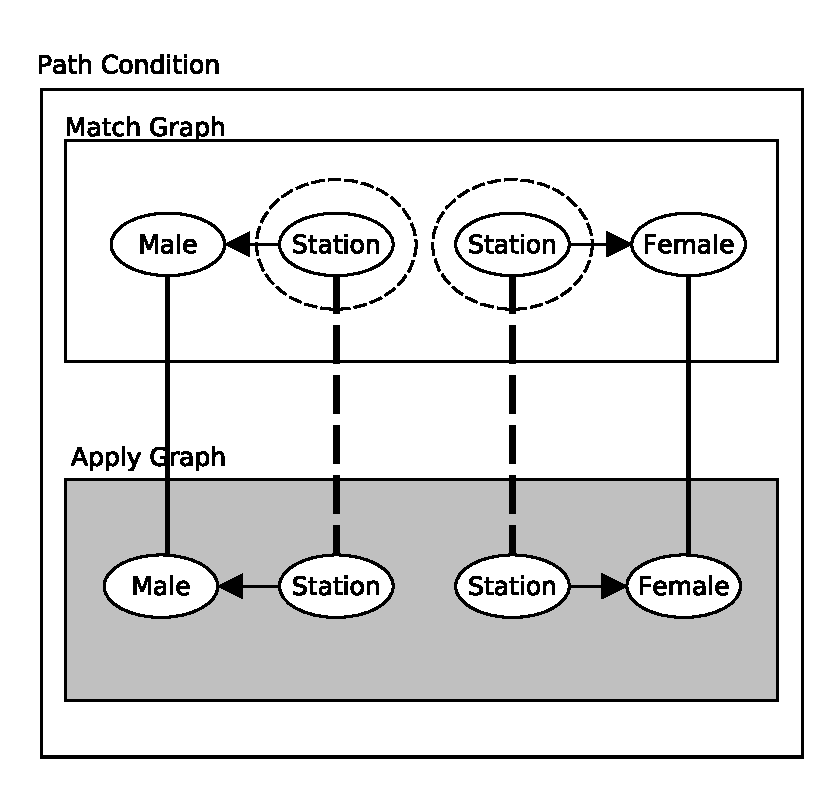
\includegraphics[width=1\textwidth]{./figures/building_path_conditions/collapse_locate_match.pdf}
                \caption{Locating two match elements}
                \label{fig:collapse_locate_match}
        \end{subfigure}%
        ~~
        \begin{subfigure}[b]{0.40\textwidth}
                \centering
                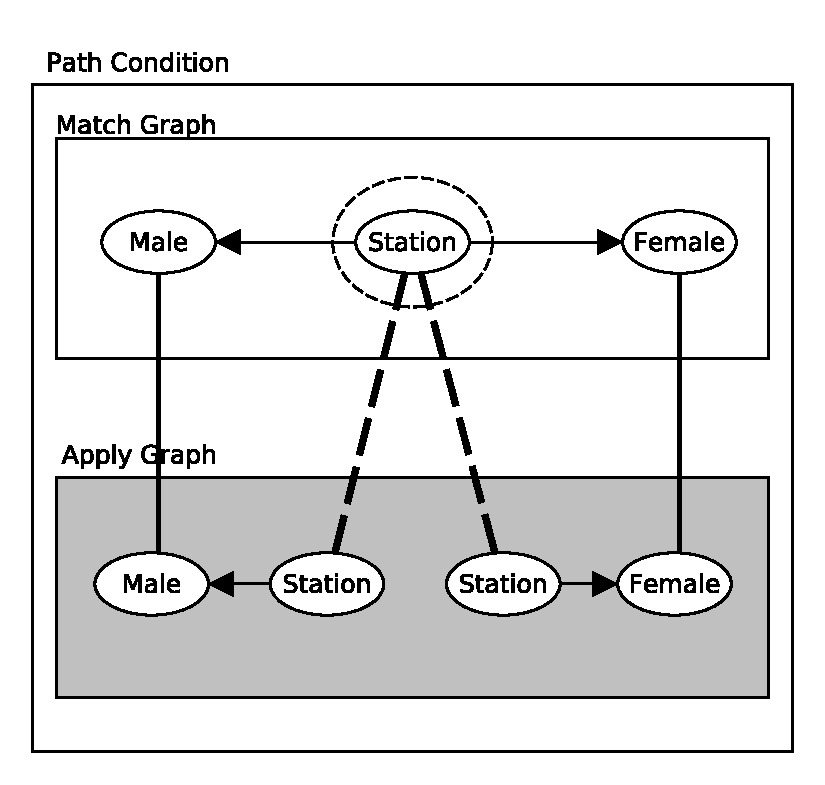
\includegraphics[width=1\textwidth]{./figures/building_path_conditions/collapse_merge_match.pdf}
                \caption{Merging the elements}
                \label{fig:collapse_merge_match}
        \end{subfigure}%
        \caption{Selecting and merging match elements of the same type}
        \label{fig:merge_match_elements}
\end{figure}


%\paragraph{Merging of Apply Elements}
%\label{para:backward_links}
%
%At this step in the disambiguation algorithm, there is a special case to be
%handled which will happen much less often than the standard step of merging only
%match elements. The algorithm must check if the two match elements just merged
%in the previous step are connected by backward links to apply elements. If there
%are two apply elements that have the same type as each other, then these apply
%elements need to be merged together in the same way as the match elements were.
%This is because the backward links indicate that these two elements were
%generated from the same match element and are therefore the same element. The
%two apply elements to be merged are highlighted in
%figure~\ref{fig:collapse_locate_apply}, and are shown merged in
%figure~\ref{fig:collapse_merge_apply}.
%

%
%  \begin{figure}[htb]
%        \centering
%        \begin{subfigure}[b]{0.40\textwidth}
%                \centering
%                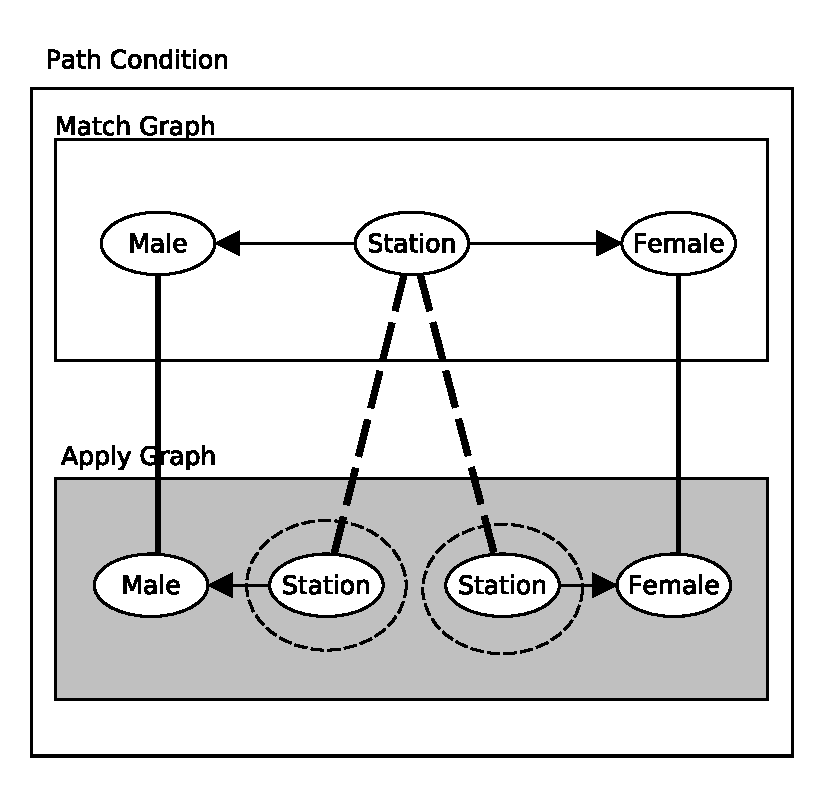
\includegraphics[width=1\textwidth]{./figures/building_path_conditions/collapse_locate_apply.pdf}
%                \caption{Locating connected apply elements}
%                \label{fig:collapse_locate_apply}
%        \end{subfigure}%
%        ~~
%        \begin{subfigure}[b]{0.40\textwidth}
%                \centering
%                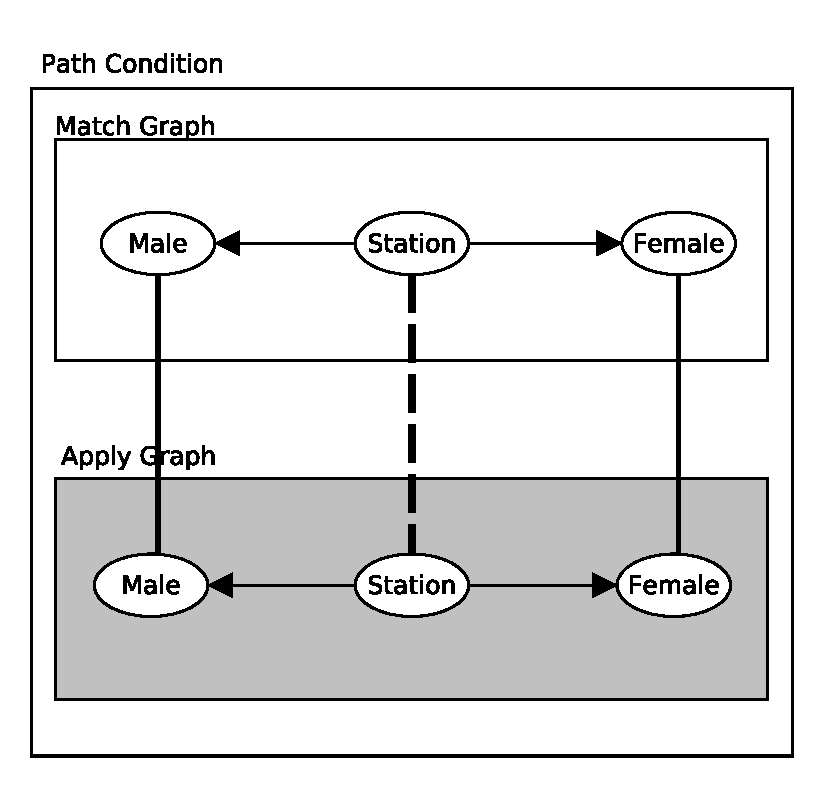
\includegraphics[width=1\textwidth]{./figures/building_path_conditions/collapse_merge_apply.pdf}
%                \caption{Merging the elements}
%                \label{fig:collapse_merge_apply}
%        \end{subfigure}%
%        \caption{Selecting and merging apply elements connected by backward links}
%        \label{fig:merge_apply_elements}
%\end{figure}

In what follows we formally define how the disambiguation of a path condition including several rules is achieved. 

\begin{definition}{Path Condition Match and Apply Element Merge Function}
\label{def:merge_apply_merge_function}

Let $pc = \big\langle V,E,st,\tau\big\rangle\in \textsc{Pathcond}^{sr}_{tg}$ be a path condition. The match element merge function $\alpha : \textsc{Pathcond}^{sr}_{tg} \rightarrow \mathcal{P}(\textsc{Pathcond}^{sr}_{tg})$ of $pc$ is such that:
\begin{align*}
\alpha(pc)=\big\{&\langle V\backslash\{y\},E',st',\tau' \rangle \;|\;\\
&\exists x,y\in Match(V)\;.\; \tau(x)=\tau(y)\;\land\; Rule(x)\setminus Rule(y) = \emptyset \;\land\\
&E'=\{x\xrightarrow{e}z\;|\;y\xrightarrow{e}z\in E_2\}\;\cup\\
&\qquad\,\,\{z\xrightarrow{e}x\;|\;z\xrightarrow{e}y\in E_2\}\;\cup\\
&\qquad\,\,\{w\xrightarrow{e}z\;|\;w\xrightarrow{e}z\in E_2 \land w\neq y \land z\neq y\}\big\}
\end{align*}

The complementary apply element merge function $\mu : \textsc{Pathcond}^{sr}_{tg}\rightarrow \mathcal{P}(\textsc{Pathcond}^{sr}_{tg})$ of $pc$ is defined as follows:
\begin{align*}
\mu(pc)=\big\{&\langle V\backslash\{y\},E',st',\tau' \rangle \;|\;\\
&\exists x,y\in Apply(V)\;.\; \tau(x)=\tau(y)\;\land\; Rule(x)\setminus Rule(y) = \emptyset \;\land\\
&\exists v\in Match(V_1)\;.\; x\xrightarrow{e} v\in E \land y\xrightarrow{e'} v\in E\;\land\; \tau(e)=\tau(e')=backward\;\land\\
&E'=\{x\xrightarrow{e}z\;|\;y\xrightarrow{e}z\in E_2\}\;\cup\\
&\qquad\,\,\{z\xrightarrow{e}x\;|\;z\xrightarrow{e}y\in E_2\}\;\cup\\
&\qquad\,\,\{w\xrightarrow{e}z\;|\;w\xrightarrow{e}z\in E_2 \land w\neq y \land z\neq y\}\big\}
\end{align*}
For the two definitions above we impose that the types of the relations that are copied from the second match/apply element to the one are preserved by the typing function $\tau'$.\\
\end{definition}

The match and apply element merge functions are complementary: the match merge function merges two match elements and the apply element merge function merges two apply elements, but only if they are connected by a backward link to the same match element.

\paragraph{Recursive Disambiguation}

In the above example, we have shown the merging of one pair of elements with the
same type in the match graph. This example has produced one path condition where no elements were merged, and one where the
\emph{Station} elements were merged.

In the general case, these produced path conditions may still be ambiguous, as
there could be further pairs of elements to be disambiguated. Therefore the
disambiguation algorithm is recursive. Every path condition produced by this
algorithm must be recursively examined for other pairs of elements to merge.

At the conclusion of the disambiguation algorithm, the final set of path
conditions will contain every possibility of merged and unmerged pairs of
elements. We then define this set to contain the \emph{unambiguous path
conditions} for the layer in question.


\begin{definition}{Path Condition Disambiguation Function}
\label{def:path_cond_disamb_function}

Let $pc = \big\langle V,E,st,\tau\big\rangle\in \textsc{Pathcond}^{sr}_{tg}$ be a path condition. The disambiguation function $disamb : \textsc{Pathcond}^{sr}_{tg}\rightarrow \mathcal{P}(\textsc{Pathcond}^{sr}_{tg})$ is recursively defined as:
\begin{gather*}
  disamb(pc) =
  \begin{cases}
    pc  & \text{if } \alpha(pc)=\emptyset \\
    pc\;\cup\;step(pc) \;\cup\;
    \bigcup_{pc'\in step(pc)} disamb(pc') & \text{if } \alpha(pc)\neq \emptyset
  \end{cases}
\end{gather*}
\center{\text{where} $step(pc) = \bigcup_{pc'\in \alpha(pc)} \mu(pc')$}
\end{definition}

As shown in definition~\ref{def:path_cond_disamb_function}, the disambiguation function returns the unchanged path condition if no match elements can be merged by function $\alpha$ ($\alpha(pc)=\emptyset$). In case match elements can be merged, the disambiguation function will return the input path condition, united with all separate possibilities of merging pairs of match (and potentially apply) elements ($step(pc)$), united with the recursive disambiguation of all those possibilities in $step(pc)$.

\begin{proposition}{The result of disambiguating a path condition is a finite set of path conditions.}
\end{proposition}

